\documentclass[12pt,twoside]{article}
\usepackage[dvipsnames]{xcolor}
\usepackage{tikz,graphicx,amsmath,amsfonts,amscd,amssymb,bm,cite,epsfig,epsf,url}
\usepackage[hang,flushmargin]{footmisc}
\usepackage[colorlinks=true,urlcolor=blue,citecolor=blue]{hyperref}
\usepackage{amsthm,multirow,wasysym,appendix}
\usepackage{array,subcaption} 
% \usepackage[small,bf]{caption}
\usepackage{bbm}
\usepackage{pgfplots}
\usetikzlibrary{spy}
\usepgfplotslibrary{external}
\usepgfplotslibrary{fillbetween}
\usetikzlibrary{arrows,automata}
\usepackage{thmtools}
\usepackage{blkarray} 
\usepackage{textcomp}
\usepackage[left=0.8in,right=1.0in,top=1.0in,bottom=1.0in]{geometry}

%% Probability operators and functions
%
% \def \P{\mathrm{P}}
\def \P{\mathrm{P}}
\def \E{\mathrm{E}}
\def \Var{\mathrm{Var}}
\let\var\Var
\def \Cov {\mathrm{Cov}} \let\cov\Cov
\def \MSE {\mathrm{MSE}} \let\mse\MSE
\def \sgn {\mathrm{sgn}}
\def \R {\mathbb{R}}
\def \C {\mathbb{C}}
\def \N {\mathbb{N}}
\def \Z {\mathbb{Z}}
\def \cV {\mathcal{V}}
\def \cS {\mathcal{S}}

\newcommand{\RR}{\ensuremath{\mathbb{R}}}

\DeclareMathOperator*{\argmin}{arg\,min}
\DeclareMathOperator*{\argmax}{arg\,max}
\newcommand{\red}[1]{\textcolor{red}{#1}}
\newcommand{\blue}[1]{\textcolor{blue}{#1}}
\newcommand{\green}[1]{\textcolor{ForestGreen}{ #1}}
\newcommand{\fuchsia}[1]{\textcolor{RoyalPurple}{ #1}}



%
%% Probability distributions
%
%\def \Bern    {\mathrm{Bern}}
%\def \Binom   {\mathrm{Binom}}
%\def \Exp     {\mathrm{Exp}}
%\def \Geom    {\mathrm{Geom}}
% \def \Norm    {\mathcal{N}}
%\def \Poisson {\mathrm{Poisson}}
%\def \Unif    {\mathrm {U}}
%
\DeclareMathOperator{\Norm}{\mathcal{N}}

\newcommand{\bdb}[1]{\textcolor{red}{#1}}

\newcommand{\ml}[1]{\mathcal{ #1 } }
\newcommand{\wh}[1]{\widehat{ #1 } }
\newcommand{\wt}[1]{\widetilde{ #1 } }
\newcommand{\conj}[1]{\overline{ #1 } }
\newcommand{\rnd}[1]{\tilde{ #1 } }
\newcommand{\rv}[1]{ \rnd{ #1}  }
\newcommand{\rM}{\rnd{ m}  }
\newcommand{\rx}{\rnd{ x}  }
\newcommand{\ry}{\rnd{ y}  }
\newcommand{\rz}{\rnd{ z}  }
\newcommand{\ra}{\rnd{ a}  }
\newcommand{\rb}{\rnd{ b}  }
\newcommand{\rt}{\rnd{ t}  }
\newcommand{\rs}{\rnd{ s}  }


\newcommand{\rpc}{\widetilde{ pc}  }
\newcommand{\rndvec}[1]{\vec{\rnd{#1}}}

\def \cnd {\, | \,}
\def \Id { I }
\def \J {\mathbf{1}\mathbf{1}^T}

\newcommand{\op}[1]{\operatorname{#1}}
\newcommand{\setdef}[2]{ := \keys{ #1 \; | \; #2 } }
\newcommand{\set}[2]{ \keys{ #1 \; | \; #2 } }
\newcommand{\sign}[1]{\op{sign}\left( #1 \right) }
\newcommand{\trace}[1]{\op{tr}\left( #1 \right) }
\newcommand{\tr}[1]{\op{tr}\left( #1 \right) }
\newcommand{\inv}[1]{\left( #1 \right)^{-1} }
\newcommand{\abs}[1]{\left| #1 \right|}
\newcommand{\sabs}[1]{| #1 |}
\newcommand{\keys}[1]{\left\{ #1 \right\}}
\newcommand{\sqbr}[1]{\left[ #1 \right]}
\newcommand{\sbrac}[1]{ ( #1 ) }
\newcommand{\brac}[1]{\left( #1 \right) }
\newcommand{\bbrac}[1]{\big( #1 \big) }
\newcommand{\Bbrac}[1]{\Big( #1 \Big)}
\newcommand{\BBbrac}[1]{\BIG( #1 \Big)}
\newcommand{\MAT}[1]{\begin{bmatrix} #1 \end{bmatrix}}
\newcommand{\sMAT}[1]{\left(\begin{smallmatrix} #1 \end{smallmatrix}\right)}
\newcommand{\sMATn}[1]{\begin{smallmatrix} #1 \end{smallmatrix}}
\newcommand{\PROD}[2]{\left \langle #1, #2\right \rangle}
\newcommand{\PRODs}[2]{\langle #1, #2 \rangle}
\newcommand{\der}[2]{\frac{\text{d}#2}{\text{d}#1}}
\newcommand{\pder}[2]{\frac{\partial#2}{\partial#1}}
\newcommand{\derTwo}[2]{\frac{\text{d}^2#2}{\text{d}#1^2}}
\newcommand{\ceil}[1]{\lceil #1 \rceil}
\newcommand{\Imag}[1]{\op{Im}\brac{ #1 }}
\newcommand{\Real}[1]{\op{Re}\brac{ #1 }}
\newcommand{\norm}[1]{\left|\left| #1 \right|\right| }
\newcommand{\norms}[1]{ \| #1 \|  }
\newcommand{\normProd}[1]{\left|\left| #1 \right|\right| _{\PROD{\cdot}{\cdot}} }
\newcommand{\normTwo}[1]{\left|\left| #1 \right|\right| _{2} }
\newcommand{\normTwos}[1]{ \| #1  \| _{2} }
\newcommand{\normZero}[1]{\left|\left| #1 \right|\right| _{0} }
\newcommand{\normTV}[1]{\left|\left| #1 \right|\right|  _{ \op{TV}  } }% _{\op{c} \ell_1} }
\newcommand{\normOne}[1]{\left|\left| #1 \right|\right| _{1} }
\newcommand{\normOnes}[1]{\| #1 \| _{1} }
\newcommand{\normOneTwo}[1]{\left|\left| #1 \right|\right| _{1,2} }
\newcommand{\normF}[1]{\left|\left| #1 \right|\right| _{\op{F}} }
\newcommand{\normLTwo}[1]{\left|\left| #1 \right|\right| _{\ml{L}_2} }
\newcommand{\normNuc}[1]{\left|\left| #1 \right|\right| _{\ast} }
\newcommand{\normOp}[1]{\left|\left| #1 \right|\right|  }
\newcommand{\normInf}[1]{\left|\left| #1 \right|\right| _{\infty}  }
\newcommand{\proj}[1]{\mathcal{P}_{#1} \, }
\newcommand{\diff}[1]{ \, \text{d}#1 }
\newcommand{\vc}[1]{\boldsymbol{\vec{#1}}}
\newcommand{\rc}[1]{\boldsymbol{#1}}
\newcommand{\vx}{\vec{x}}
\newcommand{\vy}{\vec{y}}
\newcommand{\vz}{\vec{z}}
\newcommand{\vu}{\vec{u}}
\newcommand{\vv}{\vec{v}}
\newcommand{\vb}{\vec{\beta}}
\newcommand{\va}{\vec{\alpha}}
\newcommand{\vaa}{\vec{a}}
\newcommand{\vbb}{\vec{b}}
\newcommand{\vg}{\vec{g}}
\newcommand{\vw}{\vec{w}}
\newcommand{\vh}{\vec{h}}
\newcommand{\vbeta}{\vec{\beta}}
\newcommand{\valpha}{\vec{\alpha}}
\newcommand{\vgamma}{\vec{\gamma}}
\newcommand{\veta}{\vec{\eta}}
\newcommand{\vnu}{\vec{\nu}}
\newcommand{\rw}{\rnd{w}}
\newcommand{\rvnu}{\vc{\nu}}
\newcommand{\rvv}{\rndvec{v}}
\newcommand{\rvw}{\rndvec{w}}
\newcommand{\rvx}{\rndvec{x}}
\newcommand{\rvy}{\rndvec{y}}
\newcommand{\rvz}{\rndvec{z}}
\newcommand{\rvX}{\rndvec{X}}


\newtheorem{theorem}{Theorem}[section]
% \declaretheorem[style=plain,qed=$\square$]{theorem}
\newtheorem{corollary}[theorem]{Corollary}
\newtheorem{definition}[theorem]{Definition}
\newtheorem{lemma}[theorem]{Lemma}
\newtheorem{remark}[theorem]{Remark}
\newtheorem{algorithm}[theorem]{Algorithm}

% \theoremstyle{definition}
%\newtheorem{example}[proof]{Example}
\declaretheorem[style=definition,qed=$\triangle$,sibling=definition]{example}
\declaretheorem[style=definition,qed=$\bigcirc$,sibling=definition]{application}

%
%% Typographic tweaks and miscellaneous
%\newcommand{\sfrac}[2]{\mbox{\small$\displaystyle\frac{#1}{#2}$}}
%\newcommand{\suchthat}{\kern0.1em{:}\kern0.3em}
%\newcommand{\qqquad}{\kern3em}
%\newcommand{\cond}{\,|\,}
%\def\Matlab{\textsc{Matlab}}
%\newcommand{\displayskip}[1]{\abovedisplayskip #1\belowdisplayskip #1}
%\newcommand{\term}[1]{\emph{#1}}
%\renewcommand{\implies}{\;\Rightarrow\;}



\begin{document}

\begin{center}
{\large{\textbf{Homework 3}} } \vspace{0.2cm}\\
Due October 3 at 11 pm
\\
\end{center}

\begin{enumerate}

\item (Half life)
The half life of a radioactive substance is a way to quantify how rapidly the substance decays. Given a fixed quantity of the substance, the half time is the time that it takes for it to be reduced to half (i.e. half of the radioactive particles have decayed). It is not immediately apparent why the time should be the same for any quantity. Here we'll show that it is (probabilistically) if the particles decay following an exponential distribution.  
\begin{enumerate}
\item Let $\rnd{t}$ be a random variable with a pdf of the form
\begin{align}
f_{\rnd{t}}(t) := \begin{cases}
\lambda \exp(- \lambda t), \qquad \text{if $t\geq 0$},\\
0 \qquad \text{otherwise},
\end{cases}
\end{align}
where $\lambda$ is a fixed constant. We define the half life $t_{1/2}$ as the number that satisfies $\P(\rnd{t} > t_{1/2}) = 1/2$. Compute $t_{1/2}$ in terms of $\lambda$. Then explain intuitively why this is a reasonable definition for the half life.
\subitem 
We can calculate $t_{1/2}$ in terms of $\lambda$ by plugging in $t_{1/2}$ into our random variable PDF, then integrate to get our cdf. First we integrate our pdf function:
$$
    P(\rnd{t} > t) = \int_{t_{1/2}}^\infty \text{PDF Function } = \int_{t_{1/2}}^\infty \lambda e^{-\lambda x}   = e^{-\lambda t_{1/2}}
$$Then we can manipulate with algebra to get: 

$$\frac{1}{2}= -e^{\lambda t_{1/2}} \rightarrow  \frac{ln(.5)}{-t\lambda} = t_{1/2}   \rightarrow \frac{ln(2)}{\lambda} = t_{1/2}     $$ 
This is a reasonable definition for half life and is intuitive makes as we calculated the probability that 50$\%$ of our matter would be gone. This makes sense our cdf function tells us the probability of an event up to a certain point and its calculated as $1-e^{\lambda (t-t_{1/2})}$. Since we set the other side to $\frac{1}{2}$ we effectively are asking the question, at what point does the probability equal 50$\%$ on each side? Which we have defined as $t_{1/2}$ and this works since we assumed all the particles have the same distribution. 

\item Compute $t$ such that $\P( t_{1/2} < \rnd{t} < t) = 1/4$, and express it in terms of only $t_{1/2}$. Explain why the result is consistent with the intuitive meaning of half life.
\subitem
$$\P( t_{1/2} < \rnd{t} < t) = 1-e^{\lambda(t-t{1/2})} = \frac{1}{2} - e^{\lambda t} = \frac{1}{4} \rightarrow t_{1/4} = \frac{ln(4)}{\lambda} \rightarrow t_{1/4} = 2\times t_{1/2}$$
Again, this intuitively makes sense as we are asking the question, how long would it take for our matter to be halved, and then be halved again? The function is "memory-less" and therefore, after it is halved once, the time that it takes to get halved again does not change. So the time to have $t_{1/4}$ of the matter is twice the amount of time to half the matter once, or $2\times t_{1/2}$
\item Compute $\P( \rnd{t} > k t_{1/2} )$ for any integer $k$. Again, explain why the result is consistent with the intuitive meaning of half life.
\subitem
$$
    \P( \rnd{t} > k t_{1/2} ) \text{where } k \in \mathbf{Z} = 1 - e^{-(\lambda kt_{1/2})} \rightarrow e^{ln(2^k)} = \frac{1}{2^k}
$$
The answer we derived is no surprise, as the definition of half-life is the time it takes for the mass of the radioactive quantity to be reduced by half, the time it takes to lose one half of its mass is independent of any amount of its mass it has lost until that point (it's "memory-less"). Therefore, our equation that represents half-life should be "memory-less" as well, and thus the exponential function we used to model the pdf is a great choice, as the pdf of the exponential function at time $t$ given some time $t_0$ is equivalent to the pdf exponential function shifted over $(t-t_0)$ units .
\end{enumerate}

\item (Measurements)  
You have access to the readings of a device that indicates whether a radioactive particle has decayed. However you do not get a continuous reading, you get a reading every second. 
\begin{enumerate}
\item A reasonable model for the time the particle takes to decay is that it is a random variable with pdf
\begin{align}
f_{\rnd{t}}(t) := \begin{cases}
\lambda \exp(- \lambda t), \qquad \text{if $t\geq 0$},\\
0 \qquad \text{otherwise},
\end{cases}
\end{align}
where $\lambda$ is a fixed constant. Taking into account that the measurement device rounds up the time and outputs an integer number of seconds (if the time is $0.1$ it outputs 1, if it is 13.4 it outputs 14), compute the pmf of the reading from the device. What kind of random variable is this? 
\subitem 
The pdf of this exponential random variable will be
$$
    F_{\rnd t} | \rnd t>0 (t) = \int_{(x-1)}^{x} \lambda e^{-\lambda t}dx = e^{-\lambda x-1}   - e^{-\lambda x}
$$
Which is equal to 
$$
    = (e^{-\lambda})^{x-1} \times (1-e^{-\lambda}) \text{when } x\in \mathbf{Z} \text{ when } x \geq 1
$$
\item What is the pdf of the error between your reading and the true time of decay?
\end{enumerate}
We know that when the conditional cdf of $\rnd{t}$ given $\rnd{t} \geq t_{0}$ evalutated at $t > t_{0}$ is given by:
$$
    F_{\rnd{t}|\rnd{t}>t_{0}} = P(\rnd{t}\leq t | \rnd{t} < t_0) = \frac{ e^{-\lambda }\times (e^{\lambda t -1)}}{1-e^{\lambda}} = \frac{e^{\lambda x}-1}{e^{\lambda}-1} 
$$
And if we differentiate the cdf we have obtain we get:
$$
    \frac{e^{\lambda t}-1}{e^{\lambda}-1}dt = \frac{\lambda e^{\lambda t}}{e^{\lambda} -1} 
$$
Of course, cdfs are cumulative probability functions, and only hold inbetween the values of 0 and 1, so therefore the function is only valid for that range. That is to say:
$$
    f_{\rnd t}(t) =  \begin{cases} 
      \frac{\lambda e^{\lambda t}}{e^{\lambda}-1}, & 0 \leq t \leq 1 \\
      0, & \text{in any other case}
   \end{cases}
$$

\item (Triangular pdf)
We are interested in fitting a model with a parametric pdf equal to
\begin{align}
f_{w}\brac{x}  = \begin{cases}
 \frac{2x}{w^2}, \qquad & \text{for } 0 \leq x \leq w,\\
0, \qquad & \text{otherwise},
\end{cases}
\end{align}
where the parameter $w$ is nonnegative. 
%\begin{comment}
%Both the pdf and the cdf are plotted in Figure~\ref{fig:triangle}.  
%\begin{figure}[tp]
%% Preamble: \pgfplotsset{width=7cm,compat=1.12}
%% \begin{center}
%\begin{tikzpicture}[scale=0.95]
%\begin{axis}[xmin= -0.1, xmax=2.1, ymin=-0.1, ymax=1.1,xlabel=$x$,
%ylabel=$f_{X} \brac{x }  $, xticklabels={0,w}, xtick={0,2},
%yticklabels={0,$\frac{2}{w}$}, ytick={0,1}]
%\addplot[blue, very thick, domain=0:2, samples=51] { x/2)};
%\addplot[blue, very thick, domain=-0.1:0, samples=2] {0};
%\addplot[blue, very thick, domain=2:2.1, samples=2] {0};
%\addplot[dashed, very thick, samples=2] coordinates {(2,0)(2,1)};
%\end{axis}
%\end{tikzpicture}
%%\end{center}
%\caption{Triangular pdf and the corresponding cdf.}
%\label{fig:triangle}
%\end{figure}
%\end{comment}

\begin{enumerate}
\item The observed values are 1.25, 0.4, 1.5, 1, 1.2. What are the possible values of the parameter $w$? 
\subitem $w \geq 1.5$ is the current constraint, as we fit a model to our empirical data using the maximum value of the datapoints that we observed, which is equal to $(1.5)$. Therefore $w \geq 1.5$ 
\item Compute the likelihood function corresponding to these data and sketch it. 
\subitem 
$$
\prod_{i=1}^n \frac{2_{x_i}}{w^2} \rightarrow n=5 \rightarrow \frac{2^5}{w^{10}} \prod_{i=1}^n x_i = \frac{28.8}{w^{10}} \rightarrow \text{ W is maximized at } w=1.5
$$
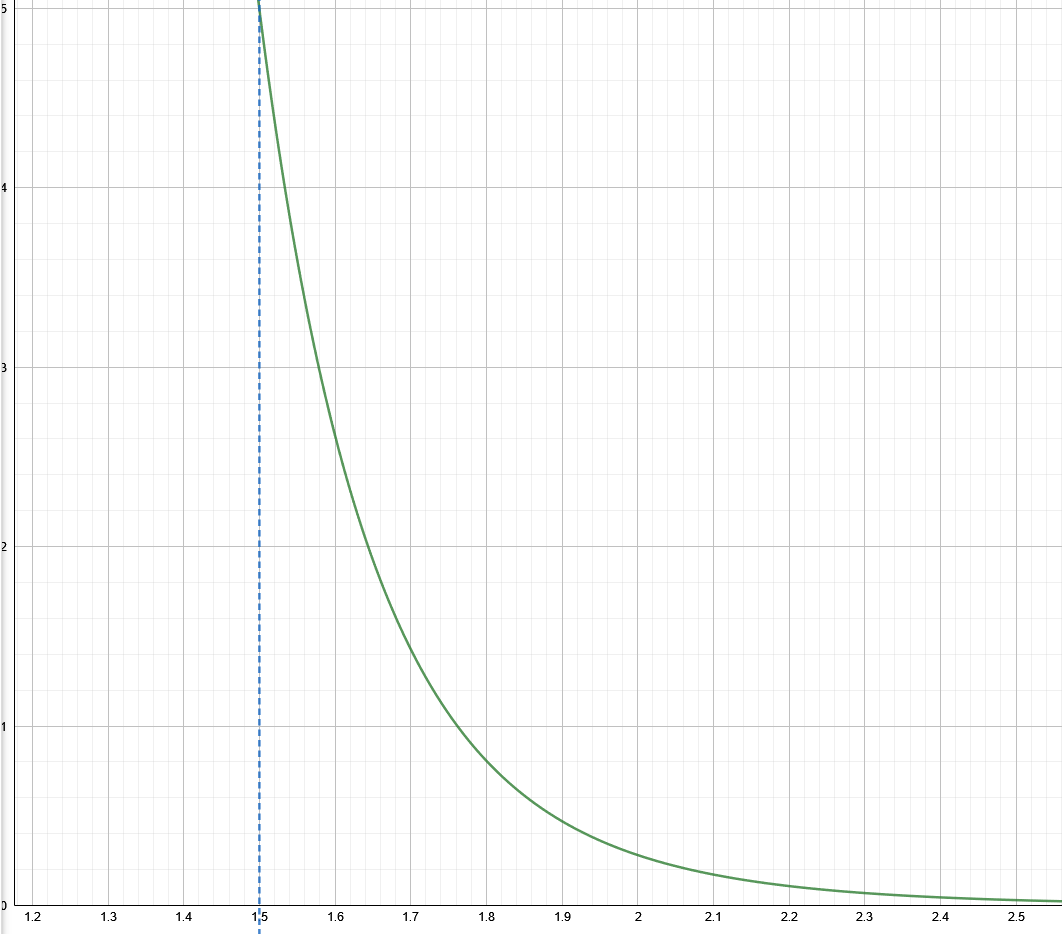
\includegraphics[scale=.34]{Hw3 graph.png}
\item What is the maximum likelihood estimate of $w$? 

Looking at the graph we can see that the maximum likelihood is $MLE = 1.5$ as our pdf is always decreasing and begins at value $w=1.5$. 

\item  If we observe 100 independent samples that are generated according to the parametric model with a fixed value of $w$, do you think that there is any chance that the ML estimate of $w$ is correct? Justify your answer intuitively.
\subitem No, its intuitive to understand that since we generated this MLE with such a small sample size, and fixed to a maximum of 1.5 as that was our MLE, it will not be representative of a other actual data points as the probability of getting those values according to our MLE will be 0$\%$.

\item Let us assume $w=2$. Generate a sample from a random variable following the model using a uniform sample from the interval $\sqbr{0,1}$ equal to 0.64. 
\subitem 
$$
    \text{Likelihood function} \rightarrow pdf \rightarrow y = \frac{2x}{w^2} = \frac{2x}{4} \rightarrow cdf = \int_{0}^1 \frac{2x}{4} = \frac{x^2}{4}
$$

$$
    \text{Get the inverse cdf } x = \frac{y^2}{4} \rightarrow y=\sqrt{4x} \text{ Evaluate from interval 0 to .64} \rightarrow \sqrt{4(.64)} -0 = 1.6
$$
\end{enumerate}

\item (Applying the cdf) The array in \texttt{samples.npy} contains 1,000 i.i.d. samples from an exponential distribution with parameter $\lambda:=1$. Let $F$ denote the cdf of this distribution. 

\begin{enumerate}
\item Apply $F$ to the data (i.e. for each data point $x$ compute $F(x)$) and plot the corresponding histogram. What shape does it have?
\subitem 
It has the shape of an approximate uniform distribution. See below:

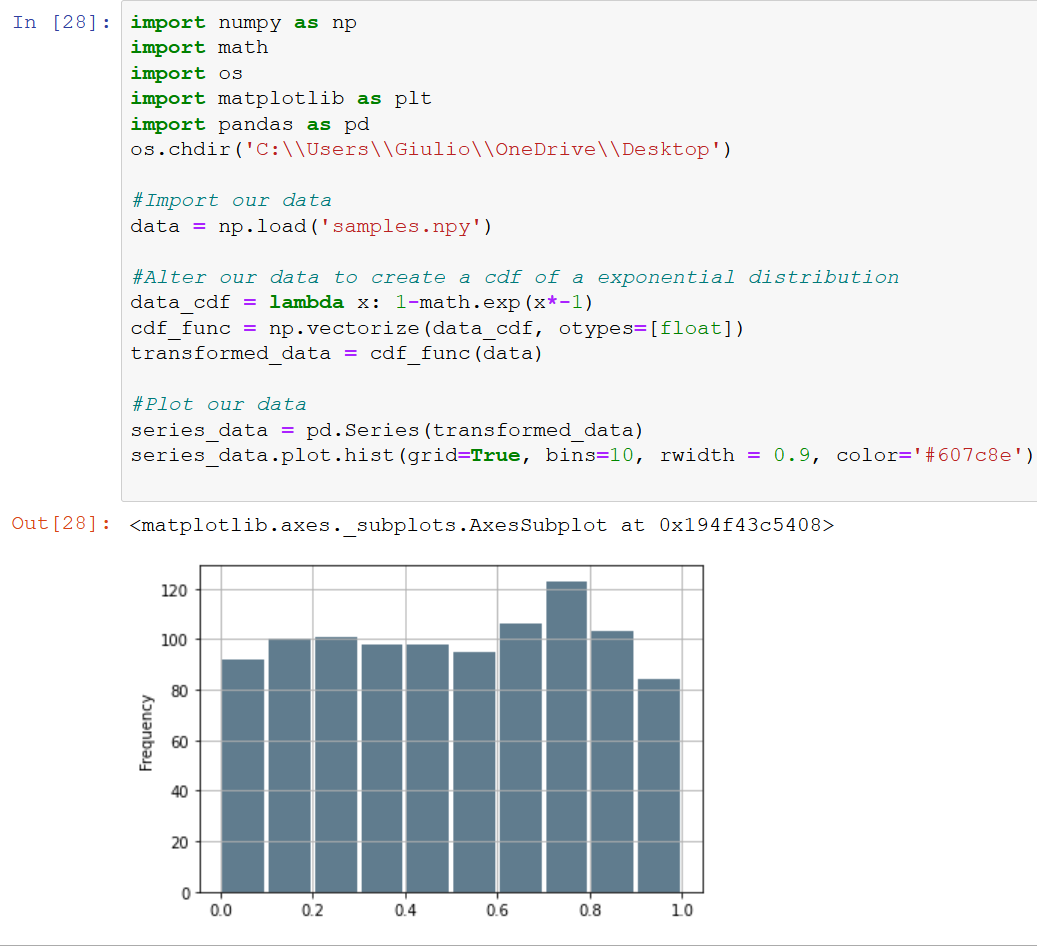
\includegraphics[scale=.5]{hw3graph2.png}
\item Let $\rnd{a}$ be a random variable with an invertible cdf $F_{\rnd{a}}$. What is the distribution of $F_{\rnd{a}}(\rnd{a})$? Justify your answer mathematically.
\subitem
We know that if a cdf is invertible it represents the cdf a continuous random variable, and due to the universality of the norm if we plug in the random variable $\rnd{a}$ into its own cdf $F_{\rnd{a}}(\rnd{a})$ then the distribution that follows will map to the points $[0,1]$ and be a uniform distribution. We can prove this property in the following way. \\

Since $F_{\rnd{a}}(\rnd{a})$ takes in values $(0,1)$, $P(F_{\rnd{a}}(\rnd{a}) \leq x)) = 0$ for $x <0$ and equals 1 for $x\geq 1$. For all $x \in (0,1)$:
$$
    P(F_{\rnd{a}}(\rnd{a}) \leq x) = P(\rnd{a} \leq F_{\rnd{a}}^{-1}(x)) = F_{\rnd{a}}(F_{\rnd{a}}^{-1}(x)) =x $$ 

Therefore $F_{\rnd{a}}(\rnd{a})$ has the univeform distribution $(0,1)$ CDF.
\end{enumerate}

\end{enumerate}
\end{document}
